\section{Odometry}

Odometry refers to the use of sensor data to estimate changes in pose over time. This can be seen as a specific instance of the more general problem of estimating some of the states of a dynamical system 

\begin{equation}
    \Dot{x} = f(x,u(t), w(t))
\end{equation}

where $x$ is the state, $u(t)$ is the input at time $t$ and $w(t)$ is the noise input. The states are measured through a measurement function

\begin{equation}
    y = h(x,v(t))
\end{equation}

where $y$ is the measurement and $v(t)$ is measurement noise. The solution depends on an initial value $x_0$ for the state. The problem is then to make an estimator for the state or part of the state that converges to the true value over time.

In the specific case met by Revolve NTNU the states we want to estimate are the linear and angular velocities, which are then to be integrated up to give an initial estimate of the change in position.

The general field of state estimation is a broad one, that has been studied extensively. Below some general state estimation algorithms and design methodologies are explained, as well as some that are more specific to our case. Some of the algorithms make more assumptions on the dynamical model, measurement function and the model and measurement noise, and thus it must be evaluated whether they fit the specific problem at hand if they are to be used. 

\subsection{Kalman filter}

One could argue that the Kalman filter is the most widely used and most successful algorithm to ever come out of the control community. It is ubiquitous, showing up in everything from cars to cell phones. What it is at its core is a way of combining sensor data and knowledge of a dynamical system, to get a better estimate of its states, even when faced with noise. 

A Kalman filter uses a dynamical model of a system, as well as knowledge of the noise that influences it, and is capable of combining several different types of sensors, making it a very powerful and easy way of doing sensor fusion. It estimates how the system will develop, propagating not only its states, but also its covariance. This makes it able to know optimally how much it should give weight to measurements compared to the estimates coming out of integrating the dynamical model. 

One main property of the Kalman filter is the so called Markov assumption. This is the assumption that the current state only depends on the previous state and the input. This is compared to a smoothing approach, where either all or at least some of the previous states are assumed to have an effect on the current state. In this case the problem is not only to find the most probable current state given the measurement, but the set of most probable states given all the measurements. 

The Kalman filter is proven to be the optimal estimator when applied to a linear system with additive zero-mean Gaussian noise, or a nonlinear system with the same noise that is linearized around its true solution. The latter is of course not possible, since if the true solution was known there would be no need to estimate the states of the system. It does however mean that if the estimate is close to the true solution, the estimator will give good results. Doing so gives an \gls{EKF}\cite{EKF}. This is the most common version of the Kalman filter, considering most systems in the real world are not truly linear systems.  

\todo[inline]{Se over dette!}

To be more specific, the Kalman filter tries to solve the problem of estimating the states of a nonlinear dynamical system with additive zero-mean Gaussian noise. It consists of a linear or linearized system with a transition matrix for each time step $k$, $F_{k}$, a way of influencing the system through the actuator $u_k$, represented as a matrix $B_{k}$, which is either the linear input function or the linearized input function. Together they give the a priori estimate of the state

\begin{equation}
    \hat{x}_{k|k-1} = F_k\hat{x}_{k-1|k-1} + B_k u_k
\end{equation}

To get the resulting distribution, one propagates the covariance through the system, to find the predicted error covariance

\begin{equation}
    P_{k|k-1} = F_k P_{k-1|k-1} F^T_{k} + Q_k
\end{equation}

where $Q_k$ is the system noise covariance, and $P_{k-1|k-1}$ is the error covariance in the previous step. The error between the measured state $z_k$ and the estimated state $H_k \hat{x}_{k|k-1}$ is then found, where $H_k$ is the linear or linearized measurement function. This error is from now on called $\Tilde{y}_k$. To find the optimal weighting between measurement and estimation, the so called Kalman gain, $K_k$, is created

\begin{equation}
    K_k = P_{k|k-1}H^T_kS^{-1}_k
\end{equation}

where 

\begin{equation}
    S_k = R_k + H_kP_{k|k-1}H^T_k
\end{equation}

is the measurement covariance, $R_k$, plus the propagated noise from the previous step. This gain is then used to give a high weight to the measurement when the measurement noise is small and system noise is large, and vice versa. The estimate of the state then is

\begin{equation}
    \hat{x}_{k|k} = \hat{x}_{k|k-1} + K_k\Tilde{y}_k
\end{equation}

To set up for the next step, the a posteriori covariance is found by

\begin{equation}
    P_{k|k} = (I-K_kH_k)P_{k|k-1}(I-K_kH_k)^T + K_kR_kK^T_k
\end{equation}

This gives an error of 

\begin{equation}
    \Tilde{y}_{k|k} = z_k - H_k\hat{x}_{k|k}
\end{equation}

which can be proven to be optimal for linear systems and around the true trajectory of linearized nonlinear systems, as is done in e.g. the original paper by Rudolf E. Kalman \cite{kalmanOG}.

\subsection{Extensions to the Kalman filter}

To deal with specific instances of the state estimation problem, extensions to the Kalman filter have been developed. 

The \gls{MEKF}\cite{MEKF} was developed to deal with the singularities that arise when rotation of a rigid three dimensional body is parametrized as three angles. 

The \gls{UKF}\cite{UKF} avoids having to linearize the dynamical system to propagate the covariance. It instead represents the state distribution as a set of particles, chosen such that they have some of the same statistical properties as the distribution they are sampled from. These are then propagated through the full nonlinear state transition function, and the new distribution is recreated using them. The resulting distribution, when this method is applied to a nonlinear system with additive zero-mean Gaussian noise is proven to be a third order approximation, compared to only a first order approximation in the \gls{EKF}. For a non-Gaussian distribution this method is still correct to the second order.

A method that manages to do state estimation of systems with more general noise characteristics is the particle filter. It was first introduced in \cite{ParticleFilter} in 1996, but not made viable before 2000, when re-sampling was introduced\cite{ParticleResampling}. It attacks the problem of state estimation from the view point that the best estimate of the state would be achieved if we had the \gls{pdf} of the state given the inputs, measurements and measurement model. But since this is not something we usually have analytically, it instead approximates it by a discrete set of particles, where the density of the particles in the state space over time will approximate the true \gls{pdf}. 

The basic principle of a particle filter is 

\begin{itemize}
    \item pulling samples (usually called particles) from a prior distribution, 
    \item weighting them with how much deviation there is from the true distribution, 
    \item normalising the weights and then re-sampling the particles (with replacement) where the probability of sampling a specific particle is its weight. 
\end{itemize}

This method is able to approximate more distributions than the Gaussian distribution the Kalman filter approximates. It does however suffer when the state space is of high dimensionality. For this reason the Rao-Blackwellized particle filter has been developed.

It assumes it is possible to partition the state, $\xi$, into two states, $\xi_1$ and $\xi_2$, that has a joint probability distribution 

\begin{equation}
    P(\xi_1,\xi_2) = P(\xi_2|\xi_1)P(\xi_1)
\end{equation}

where the conditional probability $P(\xi_2|\xi_1)$ is possible to represent analytically. This means that only $P(\xi_1)$ needs to be represented by sampling particles. The effect of this is that the marginal $P(\xi_2)$ is possible to compute with less particles, possibly making it computationally feasible.

\subsection{Smoothing}

The above state estimation methods all use the Markov assumption to marginalise the previous information. That is to say, it assumes that all states depend only on the state before it and the latest input. A contrary approach to this is to try to find the total set of state assignments that minimises the error, given all the measurements so far. This is what is known as smoothing. If instead of trying to find all the states $\{x_0,\dots,x_t\}$, one only looks at a finite amount of time back in time, i.e. only tries to find the $\{x_{t-k},...,x_{t}\}$ latest states, then this is what is called fixed-lag smoothing. The fixed-lag smoother reduces to a filter when $k=0$, of which a Kalman filter is an example.

A smoothing approach to state estimation is usually done through nonlinear optimisation. SLAM can be seen as smoothing, because usually one is not only interested in finding the latest pose, but the entire path taken so far that minimises the error between measurement and prediction. 

\subsection{Single sensor odometry}

In addition to the above mentioned state estimation approaches, there exists algorithms that try to create an odometry source through the use of only one sensor. The most prominent of these are the visual odometry that use the camera to try to estimate the relative pose between consecutive frames. This can then be used in a filter like the EKF, or in a smoothing approach. Smoothing implies not only estimating the distribution of the latest pose, but also the distribution of previous poses. 

One of the most popular single sensor odometry algorithms is \gls{SVO}\cite{SVO} and more recently its stereo extension \gls{SVO} 2.0\cite{SVO2}. It finds feature points in the two consecutive images using FAST corner detection\cite{FAST} and Edgelets edge detector\cite{Edgelet}. Only the points that can be matched between the images are kept. Around the features a patch of pixels are chosen. These patches are then transformed from one of the frames into the other using the intrinsic parameters of the camera. Then the pose that minimises the difference between the pixel value of the projected and the true pixels is found, see figure \ref{Fig:SVO}. 

\begin{figure}
    \centering
    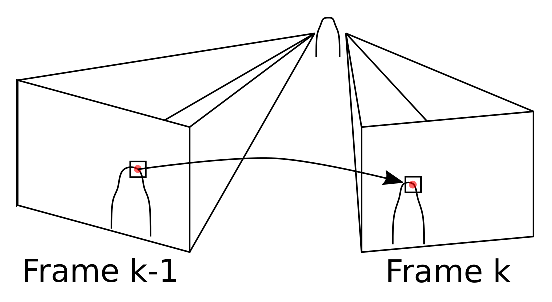
\includegraphics[width=0.8\linewidth]{0_Images/3_Background/SVO.eps}
    \caption[Illustration of \gls{SVO}'s reprojection of an image patch.]
    {Illustration of \gls{SVO}'s projection of an image patch from one image into another. It tries to find the pose that minimises the difference between the pixel value of the projected and the true pixels.}
    \label{Fig:SVO}
\end{figure}

The relative poses are then used in a smoothing approach called motion-only bundle adjustment, where the squared sum of the reprojection error for all the latest poses are minimised by nonlinear optimisation. How many poses to include in this optimisation is dependent on how much computational power is at hand and the needed output rate.

A problem with using a single camera for positioning, is that it provides no information about the absolute size of the pose changes, only relative information. This is tackled by either having something in the frame of known size that everything else can relate to, or, as in the case of \gls{SVO} 2.0, by using two cameras with a known spatial relation. It can also be dealt with by fusion with an \gls{IMU}, \gls{GPS}, wheel odometry or similar. Anything that gives information about actual distances and not just the unit-less relative pose between frames. \gls{SVO} can also be made to use \gls{IMU} data as well, thus providing two sources of scale.

\gls{SVO} and \gls{SVO} 2.0 are implemented in C++ and publicly available under a non-commercial license. 

Another viable algorithm is \gls{DSO}\cite{DSO}. It does much the same as \gls{SVO}, but instead of looking at patches of pixels around feature points, it looks at entire regions of pixels where the pixel intensity gradients is deemed large enough. From these regions it samples pixels randomly and then uses these pixel values to find the optimal relative pose. The relative poses are then used in a bundle adjustment step as well. 

The author of the original \gls{DSO} paper has a publicly available C++ implementation, but although there is a theoretical stereo extension called \gls{DSO} Stereo\cite{DSOStereo}, the only implementations of the algorithm that are publicly available is a very unstable one from someone other than the author. 

Instead of using the camera information to get an odometry source, one could apply the same set of ideas to the point cloud coming out of the \glspl{LiDAR}. This gives what is known as \gls{LiDAR} Odometry. 

The most known, publicly available, algorithm at the moment is LOAM\cite{LOAM}. It finds feature points that it can match in successive swipes of the \gls{LiDAR}, that then gives point to point distance estimates. These distance estimates are then added one by one iteratively to a set of distances, and a single step of a nonlinear optimiser tries to find the pose change between frames. Distance estimates are added until the optimisation step converges. 

\subsection{Nonlinear observer}
\iffalse
One of the first papers to treat nonlinear observer design by error linearization was \cite{FirstErrorLinNonlinObs}. 

The first type that should be mentioned is EKF, statistically motivated. 

Explain the general problem, maybe mentioning stuff like observability, different forms of stability of the observers and especially the convergence to the true value over time. 

Different types of nonlinear observers that are beneficial to mention

\begin{itemize}
    \item Observers derived by linear approximation (maybe EKF first?)
    \item Statistically motivated expanded degree observers like EKF
    \item Observers derived by error linearization
    \item High gain observers
    \item Minimum energy?
    \item Sliding mode observers?
    \item Before arriving at the main one: Observers derived through Lyapunov analysis
\end{itemize}
\fi

The term nonlinear observer refers to any dynamical system run in parallel with a dynamical system, where some or all of the internal states of the parallel system tries to match some or all the states of the original dynamical system. There are mountains of different nonlinear observers, as this is a very general term. 

To separate the different types of observers, it is beneficial to do so by how they have been derived. This makes it possible to talk about each class's general properties, their pros and cons, especially in regards to ease of derivation for a specific system, how much tuning there is and overall performance.

\subsubsection{Linear approximation}

The first that should be mentioned is the nonlinear observers derived by linear approximation of the dynamical system it is trying to represent\cite{LinearizingNonlinObs}. If this is done for a linear system 

\begin{align}
    \Dot{x} &= Ax + Bu \\
    y &= Cx
\end{align}

the resulting observer

\begin{align}
    \Dot{\hat{x}} &= A\hat{x} + Bu + L(y - \hat{y}) \\
    \hat{y} &= C\hat{x}
\end{align}

will give exponential convergence of the estimate, $\hat{x}$, to the true state, $x$, as long as $A-LC$ is Hurwitz\cite{Hurwitz}. In the case of a nonlinear system the A's, B's and C's will be the first order approximations

\begin{equation}
    A = \frac{\partial f}{\partial x}|_{x=x_0}
\end{equation}
\begin{equation}
    B = \frac{\partial f}{\partial u}|_{x=x_0}
\end{equation}
\begin{equation}
    C = \frac{\partial h}{\partial x}|_{x=x_0}
\end{equation}

where again $f$ is the state transition function and $h$ is the measurement function. This will however only give local asymptotic stability when the $A-LC$ is Hurwitz and the pair $\{A,C\}$ is observable. Many of the relevant dynamical systems do not have this property, nor is local asymptotic stability always enough, so the research community has looked for more sophisticated solutions with better properties. 

\iffalse
One of the next steps the community took was to develop the statistically motivated methods, most prominent and successful of which is the Extended Kalman filter. These methods are typically so-called expanded order observers, meaning they have more internal states than the system that it is trying to approximate the states of. In the case of the Kalman filter these internal states are $\{\hat{x},P\}$, which illustrates usual approach taken by these methods; to approximate not only the state of the system, but also the underlying probability distribution it comes from. 
\fi
\subsubsection{Nonlinear observers designed using Lyapunov analysis}

A more recent development, spearheaded in part by the research community here at NTNU, is the use of Lyapunov anaysis to develop nonlinear observers that converge asymptotically to the true state\cite{PassiveFossen}. Made first for Dynamic Positioning (DP) of large boats, it consists of starting out with an initial guess for an observer, then trying to prove its stability by Lyapunov analysis and then modifying the observer until stability can be proven. 

By Lyapunov analysis\cite{Lyapunov} is meant the process of finding a Lyapunov function candidate $V(\Tilde{x})$ that is positive definite, i.e. larger than or equal to zero for all $\Tilde{x}\neq \Vec{0}$. Here $\Tilde{x}$ is the error between the true state and the estimate. The proof is then to show that this function has the special property that

\begin{equation}
    \frac{d V(\Tilde{x})}{dt} \leq 0 \;\; \forall \hat{x}
\end{equation}

If such a Lyapunov function can be found and this property holds, then the error will always go asymptotically to zero and the observers works as desired. Other properties are also possible to derive with slight changes to the analysis formulation, but this is the main way it is used. 

One of the main reasons for choosing a nonlinear observer over a Kalman filter is that once the observer is developed it needs much less tuning than the Kalman filter. An example is the 120 covariance equations in the Kalman filter for the supply vessel discussed in \cite{PassiveFossen}, compared to the 17 gains in the nonlinear observer. Another huge benefit compared to the EKF is global asymptotic stability and sometimes local exponential stability, compared to only local asymptotic stability of the EKF. 

For a system of the form 

\begin{align}
    \Dot{x} &= f(x,u,v) \\
    y &= h(x,u,w)
\end{align}

where $x$ is the state, $u$ is the input and $v$ and $w$ are noise inputs, a good place to start for the observer design would be to simply copy the dynamics with a proportional error term, setting the noise to zero.

\begin{align}
    \Dot{\hat{x}} &= f(\hat{x}, u, 0) + K\Tilde{y} \\
    \hat{y} &= h(\hat{x}, u, 0)
\end{align}

Here $\Tilde{y} = y -  \hat{y}$ is the difference between the measured y and the estimated y. A first guess for the Lyapunov function could then be the difference in physical energy of the system when in the true state and when in the estimated state, or the quadratic sum of the error in the estimated states. 